\section{Solving Laplace's equation}
To solve the equation $\laplacian\phi=0$, assume the function $\phi$ can be separated into two functions $R$ and $\Theta$
dependent on $r$ and $\theta$ respectively such that
$$
    \phi:r,\theta\mapsto R(r)\Theta(\theta)
$$
Thus, the partial derivatives of $\phi$ would be given as
\begin{align*}
    &\pdv{\phi}{r}=R'(r)\Theta(\theta)\quad&&\pdv{\phi}{\theta}=R(r)\Theta'(\theta)\\
    &\pdv[2]{\phi}{r}=R''(r)\Theta(\theta)\quad&&\pdv[2]{\phi}{\theta}=R(r)\Theta''(\theta)
\end{align*}
Substituting these expressions into the polar form of the Laplacian derived in Section~\ref{section:POLAR-LAPLACIAN} gives
\begin{align*}
    \laplacian\phi&=\pdv[2]{\phi}{r}+\frac{1}{r}\pdv{\phi}{r}+\frac{1}{r^2}\pdv[2]{\phi}{\theta}\\
    &=R''(r)\Theta(\theta)+\frac{1}{r}R'(r)\Theta(\theta)+\frac{1}{r^2}R(r)\Theta''(\theta)=0
\end{align*}
Consequently the expressions can be separated as:
\begin{align*}
    r^2R''(r)\Theta(\theta)+rR'(r)\Theta(\theta)+R(r)\Theta''(\theta)&=0\\
    r^2\frac{R''(r)}{R(r)}+r\frac{R'(r)}{R(r)}+\frac{\Theta''(\theta)}{\Theta(\theta)}&=0\\
    \implies r^2\frac{R''(r)}{R(r)}+r\frac{R'(r)}{R(r)}=-\frac{\Theta''(\theta)}{\Theta(\theta)}
\end{align*}
Then, let $\lambda\in\mathbb{R}$ be such that
\begin{align}
    \label{equation:laplace-equation:1}\lambda&=r^2\frac{R''(r)}{R(r)}+r\frac{R'(r)}{R(r)}\\
    \label{equation:laplace-equation:2}-\lambda&=\frac{\Theta''(\theta)}{\Theta(\theta)}
\end{align}

\subsection{Solving for $\Theta$}\label{section:laplace:theta}
Through \eqref{equation:laplace-equation:2} it can be shown that
\begin{align}
    \notag\frac{\Theta''(\theta)}{\Theta(\theta)}&=-\lambda\\
    \label{equation:laplace-equation:3}\implies\Theta''(\theta)+\lambda\Theta(\theta)&=0
\end{align}
Since $\Theta$ must be periodic such that $\Theta(\theta)=\Theta(\theta+2\pi)$, one function fitting this differential equation is
the complex exponential equation
\begin{equation}
    \label{equation:laplace-equation:4}\Theta:\theta\mapsto Ce^{\mu\theta}
\end{equation}
Where $C$ is some complex constant and $\mu\in\mathbb{C}$ such that $\imaginary(\mu)\neq0$. Taking the second derivative of \eqref{equation:laplace-equation:4} with respect to $\theta$ using the chain rule,
$$
    \dv[2]{\Theta}{\theta}=C\mu^2e^{\mu\theta}
$$
Thus, for the equation to satisfy \eqref{equation:laplace-equation:3}, $\mu=\pm\sqrt{-\lambda}=\pm i\sqrt{\lambda}$. To ensure
$\imaginary(\mu)\neq0$, thereby keeping $\Theta$ periodic, $\lambda>0$.
$$
    \Theta:\theta\mapsto Ce^{\pm i\sqrt{\lambda}\theta}
$$
Since the two solutions are distinct, the general solution is the linear combination of them,
\begin{align*}
    \Theta:\theta\mapsto C_1e^{i\sqrt{\lambda}\theta}+C_2e^{-i\sqrt{\lambda}\theta}\qc C_1,C_2\in\mathbb{C}
\end{align*}
By applying Euler's formula ($e^{i\alpha}=\cos\alpha+i\sin\alpha$) and some trigonometric identities it can be shown that
\begin{align*}
    C_1e^{i\sqrt{\lambda}\theta}+C_2e^{-i\sqrt{\lambda}\theta}&=C_1\left(\cos\left(\sqrt{\lambda}\theta\right)+i\sin\left(\sqrt{\lambda}\theta\right)\right)+C_2\left(\cos\left(-\sqrt{\lambda}\theta\right)+i\sin\left(-\sqrt{\lambda}\theta\right)\right)\\
    &=C_1\cos\left(\sqrt{\lambda}\theta\right)+C_1i\sin\left(\sqrt{\lambda}\theta\right)+C_2\cos\left(\sqrt{\lambda}\theta\right)-C_2i\sin\left(\sqrt{\lambda}\theta\right)\\
    &=\left(C_1+C_2\right)\cos\left(\sqrt{\lambda}\theta\right)+\left(C_1-C_2\right)i\sin\left(\sqrt{\lambda}\theta\right)
\end{align*}
Defining the constants $A=C_1+C_2$ and $B=(C_1-C_2)i$ leads to the definition of $\Theta$ as
$$
    \Theta:\theta\mapsto A\cos\left(\sqrt{\lambda}\theta\right)+B\sin\left(\sqrt{\lambda}\theta\right)
$$
Finally, to ensure the periodicity of $\Theta$, $\sqrt{\lambda}$ must be an integer, which will be called $n\in\mathbb{N}$, leading to the discrete solutions of $\Theta_n$ as
\begin{equation}\label{equation:laplace-equation:9}
    \Theta_n:\theta\mapsto A\cos\left(n\theta\right)+B\sin\left(n\theta\right)
\end{equation}

\subsection{Solving for $R$}
Rearranging \eqref{equation:laplace-equation:3} shows that
\begin{align}
   \notag r^2\frac{R''(r)}{R(r)}+r\frac{R'(r)}{R(r)}&=\lambda\\
    \label{equation:laplace-equation:8}\implies r^2R''(r)+rR'(r)-\lambda R(r)&=0
\end{align}
This type of differential equation, known as a Cauchy--Euler equation, can be solved using Frobenius method, which has the goal of finding a power series such that
\begin{equation}
    \label{equation:laplace-equation:5}R:r\mapsto\sum_{k=0}^\infty C_k r^{k+s}\qc C_0\neq0
\end{equation}
The first and second order derivatives of \eqref{equation:laplace-equation:5} are given by
\begin{align*}
    \dv{R}{r}&=\sum_{k=0}^\infty(k+s)C_k r^{k+s-1}\\
    \dv[2]{R}{r}&=\sum_{k=0}^\infty(k+s)(k+s-1)C_k r^{k+s-2}
\end{align*}
Consequently,
\begin{align}
    \label{equation:laplace-equation:6}rR'(r)&=\sum_{k=0}^\infty(k+s)C_k r^{k+s}\\
    \label{equation:laplace-equation:7}r^2R''(r)&=\sum_{k=0}^\infty(k+s)(k+s-1)C_k r^{k+s}
\end{align}
Let $C_k r^{k+s}$ be called $\sigma$ temporarily. Substituting the equations of \eqref{equation:laplace-equation:6} and
\eqref{equation:laplace-equation:7} back into \eqref{equation:laplace-equation:8},
\begin{align*}
    \sum_{k=0}^\infty(k+s)(k+s-1)\sigma+\sum_{k=0}^\infty(k+s)\sigma-\lambda\sum_{k=0}^\infty\sigma&=0\\
    \implies\sum_{k=0}^\infty(k+s)(k+s-1)\sigma+(k+s)\sigma-\lambda\sigma&=0
\end{align*}
Let $\mu=k+s$,
\begin{align*}
    0&=\sum_{k=0}^\infty\mu(\mu-1)\sigma+\mu\sigma-\lambda\sigma\\
    &=\sum_{k=0}^\infty\sigma\left(\mu(\mu-1)+\mu-\lambda\right)\\
    &=\sum_{k=0}^\infty\sigma\left(\mu^2-\lambda\right)\\
\end{align*}
Therefore,
$$
    \sum_{k=0}^\infty C_k r^{k+s}(\mu^2-\lambda)=0\qc C_0\neq0
$$
Thus, for the equation to hold when $k=0$,
\begin{align*}
    \mu^2-\lambda&=0\\
    \implies\pm\sqrt{\lambda}&=\mu\\
    &=k+s\\
    &=s
\end{align*}
Using the definition of $n=\sqrt{\lambda}$ from Section~\ref{section:laplace:theta},
\begin{align*}
    0+s&=\pm n\\
    \implies s&=\pm n
\end{align*}
For the cases $k>0$, to ensure the equation holds, because the term $(k+s)^2-\lambda$ will no longer be $0$, $C_k r^{k+s}=0$. Therefore, all terms but $k=0$ must vanish, meaning that
$$
    R:r\mapsto C_0r^{\pm n}
$$
Since $n\in\mathbb{N}$\referto{Section}{section:laplace:theta}, these solutions are distinct, and therefore the general solution is the linear combination of them,
\begin{equation}\label{equation:laplace-equation:8}
    R_n:r\mapsto ar^n+br^{-n}
\end{equation}
Where $a$ and $b$ are some real constants.

\subsection{The equation of the velocity potential \& velocity field}\label{section:THE-FORMULAE}
\subsubsection{In polar coordinates}\label{section:VELOCITY:POLAR}
Finally, the equation of the velocity potential $\phi$ can be derived by combining the equation of $\Theta_n$ from \eqref{equation:laplace-equation:9}
and $R_n$ from \eqref{equation:laplace-equation:8},
\begin{align*}
    \phi_n:r,\theta&\mapsto R_n(r)\Theta_n(\theta)\\
    \implies\phi_n:r,\theta&\mapsto\left(ar^n+\frac{b}{r^n}\right)\left(A\cos n\theta+B\sin n\theta\right)
\end{align*}
The values of the constants $a,b,A,B$, and $n$ must now be determined such that they satisfy the boundary equations, which were 
\begin{align*}
    \gradient{\phi}&=U(\rhat\cos\theta-\thetahat\sin\theta) &&\text{as $r\rightarrow\infty$}\\
    \pdv{\phi}{r}&=0                                        &&\text{when $r=L$}
\end{align*}
Computing the partial derivatives of $\phi$,
\begin{align*}
    \pdv{\phi_n}{r}&=\left(anr^{n-1}-\frac{nb}{r^{n+1}}\right)\left(A\cos n\theta+B\sin n\theta\right)\\
    &=n\left(ar^{n-1}-\frac{b}{r^{n+1}}\right)\left(A\cos n\theta+B\sin n\theta\right)\\
    \pdv{\phi_n}{\theta}&=\left(ar^n+\frac{b}{r^n}\right)\left(-An\sin n\theta+Bn\cos n\theta\right)\\
    &=n\left(ar^n+\frac{b}{r^n}\right)\left(B\cos n\theta-A\sin n\theta\right)\\
\end{align*}
Therefore, using the polar coordinate form of the gradient derived in Section~\ref{section:polar-gradient},
\begin{align*}
    \nabla\phi_n&=\pdv{\phi_n}{r}\rhat+\frac{1}{r}\pdv{\phi_n}{\theta}\thetahat\\
    &=n\left(ar^{n-1}-\frac{b}{r^{n+1}}\right)\left(A\cos n\theta+B\sin n\theta\right)\rhat+\frac{n}{r}\left(ar^n+\frac{b}{r^n}\right)\left(B\cos n\theta-A\sin n\theta\right)\thetahat\\
    &=n\left[\left(ar^{n-1}-\frac{b}{r^{n+1}}\right)\left(A\cos n\theta+B\sin n\theta\right)\rhat+\left(ar^{n-1}+\frac{b}{r^{n+1}}\right)\left(B\cos n\theta-A\sin n\theta\right)\thetahat\right]\\
\end{align*}
Considering the case where $n=1$,
\begin{align*}
    \nabla\phi_1&=\left(ar^{1-1}-\frac{b}{r^{1+1}}\right)\left(A\cos\theta+B\sin\theta\right)\rhat+\left(ar^{1-1}+\frac{b}{r^{1+1}}\right)\left(B\cos\theta-A\sin\theta\right)\thetahat\\
    &=\left(a-\frac{b}{r^{2}}\right)\left(A\cos\theta+B\sin\theta\right)\rhat+\left(a+\frac{b}{r^{2}}\right)\left(B\cos\theta-A\sin\theta\right)\thetahat
\end{align*}
As $r\rightarrow\infty$,
\begin{align*}
    \lim_{r\rightarrow\infty}\nabla\phi_1&=\left(a-\frac{b}{\infty^2}\right)\left(A\cos\theta+B\sin\theta\right)\rhat+\left(a+\frac{b}{\infty^2}\right)\left(B\cos\theta-A\sin\theta\right)\thetahat\\
    &=\left(a-0\right)\left(A\cos\theta+B\sin\theta\right)\rhat+\left(a+0\right)\left(B\cos\theta-A\sin\theta\right)\thetahat\\
    &=a\left(\left(A\cos\theta+B\sin\theta\right)\rhat+\left(B\cos\theta-A\sin\theta\right)\thetahat\right)
\end{align*}
To match the first boundary equation which was $U(\rhat\cos\theta-\thetahat\sin\theta)$ as $r\rightarrow\infty$, the value of the variables must be
\begin{align*}
    \nabla\phi_1&\left\{\begin{matrix}
        a=U\\
        b\in\mathbb{R}\\
        A=1\\
        B=0
    \end{matrix}\right.\\
    \leadsto\lim_{r\rightarrow\infty}\nabla\phi_1&=U\left(\left(\cos\theta+0\sin\theta\right)\rhat+\left(0\cos\theta-1\sin\theta\right)\thetahat\right)\\
    &=U\left(\rhat\cos\theta-\thetahat\sin\theta\right)
\end{align*}
Now consider the value of $\pdv*{\phi_1}{r}$ when $r=L$,
\begin{align*}
    \eval{\pdv{\phi_1}{r}}_{r=L}&=\left(Ur^{1-1}-\frac{b}{r^{1+1}}\right)\left(\cos\theta+0\sin\theta\right)\\
    &=\left(U-\frac{b}{r^{2}}\right)\cos\theta
\end{align*}
The second boundary equation stated that $\pdv*{\phi_1}{r}=0$ when $r=L$, therefore $b=U^2$. Thus, for the case $n=1$, it has been demonstrated that
\begin{align*}
    \nabla\phi_1&\left\{\begin{matrix}
        a=U\\
        b=UL^2\\
        A=1\\
        B=0
    \end{matrix}\right.\\
    \implies\phi_1:r,\theta&\mapsto U\left(r+\frac{L^2}{r}\right)\cos\theta\\
    \implies\vec{V}_1:r,\theta\mapsto\nabla\phi_1&=\rhat\left(U-\frac{UL^2}{r^{2}}\right)\cos\theta-\thetahat\left(U+\frac{UL^2}{r^{2}}\right)\sin\theta
\end{align*}
Since this equation matches the boundary equations perfectly, the case of $n=1$ is accepted as the principal solution. Lastly, to avoid undefined behaviour inside the cylinder, let the velocity of the fluid be defined as $\vec{0}$ when $r<L$.
\begin{equation}\label{equation:VELOCITY:POLAR}
    \vec{V}:r,\theta\mapsto\left\{\begin{matrix}
        \rhat\left(U-\frac{UL^2}{r^{2}}\right)\cos\theta-\thetahat\left(U+\frac{UL^2}{r^{2}}\right)\sin\theta&r\geq L\\
        \vec{0}&r<L
    \end{matrix}\right.
\end{equation}

\subsubsection{In Cartesian coordinates}\label{section:VELOCITY:CARTESIAN}
Finally, to convert back to Cartesian coordinates, $r$ is equivalent to the magnitude of the vector pointing from the origin to a point on the graph, $\sqrt{x^2+y^2}$. For the angular part, since the velocity potential is only dependent
on $\cos\theta$, consider its geometric definition, as illustrated in Figure~\ref{figure:TRIGENOMETRY}. 
\begin{figure}
    \begin{center}        
        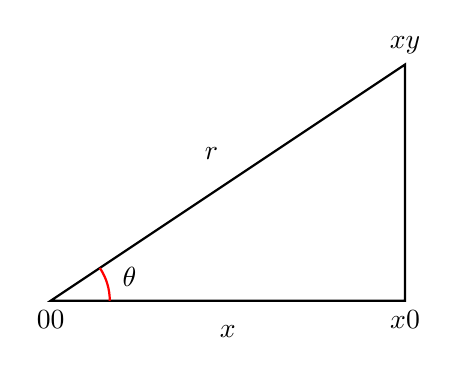
\begin{tikzpicture}[scale=0.75]
            \draw [thick] (0,0) node[anchor=north]{$\point{0}{0}$}
            -- (6,0) node[anchor=north]{$\point{x}{0}$}
            -- (6,4) node[anchor=south]{$\point{x}{y}$}
            -- cycle;
            \draw [color=red, thick] (1,-1) ++({1*cos(90)},{1*sin(90)}) 
                arc [start angle=0, end angle=33.69,
                            x radius=1, y radius=1];
            \node [right] at (1.05,0.4) {$\theta$};
            \node [below] at (3,-0.25) {$x$};
            \node [left] at (3,2.5) {$r$};
        \end{tikzpicture}
    \end{center}
    \label{figure:TRIGENOMETRY}
    \caption{Geometric definition of the trigonometric functions, with polar- and Cartesian-coordinates overlaid on a right-angled triangle}
\end{figure}
Cosine is defined as the ratio between the adjacent side ($x$) and hypotenuse ($r$) in a triangle, thus, $\cos\theta=\frac{x}{r}=\frac{x}{\sqrt{x^2+y^2}}$. Substituting this into the equation of the velocity potential gives
\begin{align*}
    \phi:x,y&\mapsto\left(Ur+\frac{UL^2}{r}\right)\cos\theta\\
    &=\left(U\sqrt{x^2+y^2}+\frac{UL^2}{\sqrt{x^2+y^2}}\right)\frac{x}{\sqrt{x^2+y^2}}\\
    &=Ux+\frac{UL^2x}{x^2+y^2}
\end{align*}
The partial derivative of $\phi$ with respect to $x$ can be computed using the quotient rule:
\begin{align*}
    \pdv{\phi}{x}&=U+UL^2\frac{x^2+y^2-x(2x)}{\left(x^2+y^2\right)^2}\\
    &=U\left(1+L^2\frac{y^2-x^2}{\left(x^2+y^2\right)^2}\right)
\end{align*}
And for the partial derivative of $\phi$ with respect to $y$, the chain rule can be applied, giving:
\begin{align*}
    \pdv{\phi}{y}&=0+UL^2x\pdv{y}\left(x^2+y^2\right)^{-1}\\
    &=-UL^2x(2y)\left(x^2+y^2\right)^{-2}\\
    &=-UL^2\frac{2xy}{(x^2+y^2)^2}
\end{align*}
Therefore, the velocity field in a Cartesian coordinate system must be given by the equation
\begin{equation}\label{equation:VELOCITY:CARTESIAN} 
    \vec{V}:x,y\mapsto\left\{\begin{matrix}
        U\left(1+L^2\frac{y^2-x^2}{\left(x^2+y^2\right)^2}\right)\ihat-UL^2\frac{2xy}{(x^2+y^2)^2}\jhat&x^2+y^2\geq L^2\\
        \vec{0}&x^2+y^2<L^2
    \end{matrix}\right.
\end{equation}

\section{The pressure field}
With the velocity field derived, the pressure field too can be derived through the Bernoulli equation,
which states for an incompressible fluid with density $\rho$ that
\begin{equation}\label{equation:BERNOULLI}
    P+\frac{\rho v^2}{2}=C
\end{equation}
Note that the term $v$ in the Bernoulli equation representing speed is scalar valued, not vector valued.
To find the value of the constant $C$, the pressure field is evaluated at a point at which the pressure
is known. At the points $r\rightarrow\infty$, the steady flow must lead to uniform pressure, denoted
$P_\infty$ and the speed at these points was defined as $U$\referto{Section}{section:INFINITELY-FAR-AWAY},
therefore
\begin{equation}\label{equation:PRESSURE}
    P_\infty+\frac{\rho U^2}{2}=C
\end{equation}
Substituting \eqref{equation:PRESSURE} into \eqref{equation:BERNOULLI},
\begin{align*}
    P+\frac{\rho v^2}{2}&=P_\infty+\frac{\rho U^2}{2}\\
    \implies P&=P_\infty+\frac{\rho U^2}{2}-\frac{\rho v^2}{2}\\
    &=P_\infty+\frac{\rho}{2}\left(U^2-v^2\right)
\end{align*}
Thus for a polar coordinate system, using the velocity field derived in \eqref{equation:VELOCITY:POLAR}\referto{Section}{section:VELOCITY:POLAR},
\begin{align}
    \notag P:r,\theta&\mapsto P_\infty+\frac{\rho}{2}\left(U^2-\lVert\vec{V}(r,\theta)\rVert^2\right)\\
    \notag\lVert\vec{V}(r,\theta)\rVert^2&=\left(U-\frac{UL^2}{r^{2}}\right)^2\cos^2\theta+\left(U+\frac{UL^2}{r^{2}}\right)^2\sin^2\theta\\
    \notag&=\left(U^2-\frac{2U^2L^2}{r^2}+\frac{U^2L^4}{r^4}\right)\cos^2\theta+\left(U^2+\frac{2U^2L^2}{r^2}+\frac{U^2L^4}{r^4}\right)\sin^2\theta\\
    \notag&=U^2\left(\cos^2\theta+\sin^2\theta\right)+\frac{U^2L^4}{r^4}\left(\cos^2\theta+\sin^2\theta\right)-\frac{2U^2L^2}{r^2}\cos^2\theta+\frac{2U^2L^2}{r^2}\sin^2\theta\\
    \notag&=U^2+\frac{U^2L^4}{r^4}-\frac{2U^2L^2}{r^2}\left(\cos^2\theta-\sin^2\theta\right)\\
    \notag&=U^2\left(1+\frac{L^4}{r^4}-\frac{2L^2}{r^2}\cos2\theta\right)\iff r\geq L\\
    \notag\lVert\vec{V}(r,\theta)\rVert^2&=0\iff r<L\\
    \notag\implies P:r,\theta&\mapsto\left\{\begin{matrix}
        P_\infty+\frac{\rho}{2}\left(U^2-\left[U^2+\frac{U^2L^4}{r^4}-\frac{2U^2L^2}{r^2}\cos2\theta\right]\right) & r\geq L\\
        P_\infty+\frac{\rho}{2}\left(U^2-0\right) & r<L
    \end{matrix}\right.\\
    \label{equation:pressure:1}&=\left\{\begin{matrix}
        P_\infty+U^2\left(\frac{L^2}{r^2}\cos2\theta-\frac{L^4}{2r^4}\right) & r\geq L\\
        P_\infty+\frac{\rho U^2}{2} & r<L
    \end{matrix}\right.
\end{align}
To convert the pressure field to a Cartesian coordinate system, recall that $r=\sqrt{x^2+y^2}$, then substitute into \eqref{equation:pressure:1},
\begin{align}
    \notag P_\infty+\rho\left(\frac{U^2L^2}{r^2}\cos2\theta-\frac{U^2L^4}{2r^4}\right)&=P_\infty+\rho\left(\frac{U^2L^2}{\sqrt{x^2+y^2}^2}\cos2\theta-\frac{U^2L^4}{2\sqrt{x^2+y^2}^4}\right)\\
    \label{equation:pressure:2}&=P_\infty+\rho\left(\frac{U^2L^2}{x^2+y^2}\cos2\theta-\frac{U^2L^4}{2\left(x^2+y^2\right)^2}\right)
\end{align}
To convert the term $\cos2\theta=\cos^2\theta-\sin^2\theta$, consider again the geometric interpretation illustrated in Figure~\ref{figure:TRIGENOMETRY},
it then follows that
\begin{align*}
    \cos\theta&=\frac{x}{r}=\frac{x}{\sqrt{x^2+y^2}}\\
    \sin\theta&=\frac{y}{r}=\frac{y}{\sqrt{x^2+y^2}}
\end{align*}
Consequently,
\begin{align}
    \notag\cos2\theta&=\left(\frac{x}{\sqrt{x^2+y^2}}\right)^2-\left(\frac{y}{\sqrt{x^2+y^2}}\right)^2\\
    \label{equation:pressure:3}&=\frac{x^2-y^2}{\sqrt{x^2+y^2}^2}=\frac{x^2-y^2}{x^2+y^2}
\end{align}
Substituting \eqref{equation:pressure:3} into \eqref{equation:pressure:2} and setting up the piecewise function definition,
\begin{align*}
    P_\infty+\rho\left(\frac{U^2L^2}{r^2}\cos2\theta-\frac{U^2L^4}{2r^4}\right)&=P_\infty+\rho\left(\frac{U^2L^2}{x^2+y^2}\frac{x^2-y^2}{x^2+y^2}-\frac{U^2L^4}{2\left(x^2+y^2\right)^2}\right)\\
    &=P_\infty+\rho\left(\frac{U^2L^2\left(x^2-y^2\right)}{\left(x^2+y^2\right)^2}-\frac{U^2L^4}{2\left(x^2+y^2\right)^2}\right)\\
    &=P_\infty+U^2\rho\left(\frac{2L^2\left(x^2-y^2\right)-L^4}{2\left(x^2+y^2\right)^2}\right)\\
    \implies P:x,y&\mapsto\left\{\begin{matrix}
        P_\infty+U^2\rho\left(\frac{2L^2\left(x^2-y^2\right)-L^4}{2\left(x^2+y^2\right)^2}\right) & x^2+y^2\geq L^2\\
        P_\infty+\frac{\rho U^2}{2} & x^2+y^2<L^2
    \end{matrix}\right.
\end{align*}